\section{Goals}

\begin{frame}[t]
	\frametitle{Goals}

	\vfill
	{\fontsize{10}{6}
		How to define the \texttt{GSpline} type:
		\begin{itemize}
			\item Represent Minimum-X and more generic trajectories
			\item Use a minimal set of math axioms
			\item Return the same time after the following operations
			      \begin{itemize}
				      \item Derivatives
				      \item Elementary linear operations
				      \item Linear Scaling
			      \end{itemize}
		\end{itemize}
	}
	\vfill
\end{frame}

\begin{frame}[t]
	\frametitle{Goals: Fundamental Axioms}
	{\fontsize{9}{5}
		\begin{itemize}
			\item defining Analytic operations (Analytical consistency)
			      \begin{equation*}
				      \diffk{}{t}{k}:\text{GSpline}\longrightarrow \text{GSpline}
			      \end{equation*}
			\item to define algebraic operations
			      \begin{eqnarray*}
				      +:\text{GSpline}\longrightarrow \text{GSpline}\\
				      \cdot:\mathbb{R} \times \text{GSpline}\longrightarrow \text{GSpline}
			      \end{eqnarray*}
			\item Linear Scaling
			      \begin{eqnarray*}
				      \left[t \rightarrow \sigma t \right]:\text{GSpline}\longrightarrow \text{GSpline}
			      \end{eqnarray*}
		\end{itemize}
		It's essential that these operations are closed within the same class: that is, performing any of these operations on instances of \Verb|GSpline| should result in another \Verb|GSpline| object
	}
\end{frame}
\begin{frame}[t]
	\frametitle{Goals: Monoid property}

	{\fontsize{10}{5}
		A \textbf{monoid} is an algebraic structure consisting of a set $M$ equipped with a binary operation
		$ \ast : M \times M \to M $ that satisfies the following properties:

		1. \textbf{Closure}:
		\begin{eqnarray*}
			\forall a, b \in M, \quad a \ast b \in M
		\end{eqnarray*}

		2. \textbf{Associativity}:
		\begin{eqnarray*}
			\forall a, b, c \in M, \quad (a \ast b) \ast c = a \ast (b \ast c)
		\end{eqnarray*}

		3. \textbf{Identity Element}:
		\begin{eqnarray*}
			\exists e \in M \text{ such that } \forall a \in M, \quad e \ast a = a \ast e = a
		\end{eqnarray*}

	}
\end{frame}
\begin{frame}[t]
	\frametitle{Goals: Monoid property}
	\begin{itemize}
		\item We desire to achieve the monoid property on the derivative, scaling and addition/scalar multiplication operations. These operation will become a monoid under the composition.
		\item Composition is a fundamental tool in programming, the Monoid structure is the most fundamental compositional structure
	\end{itemize}
	\vskip 1cm
	\begin{center}
		
\includegraphics[height=0.2\textwidth]{./images/ccpconMonoids.png}
		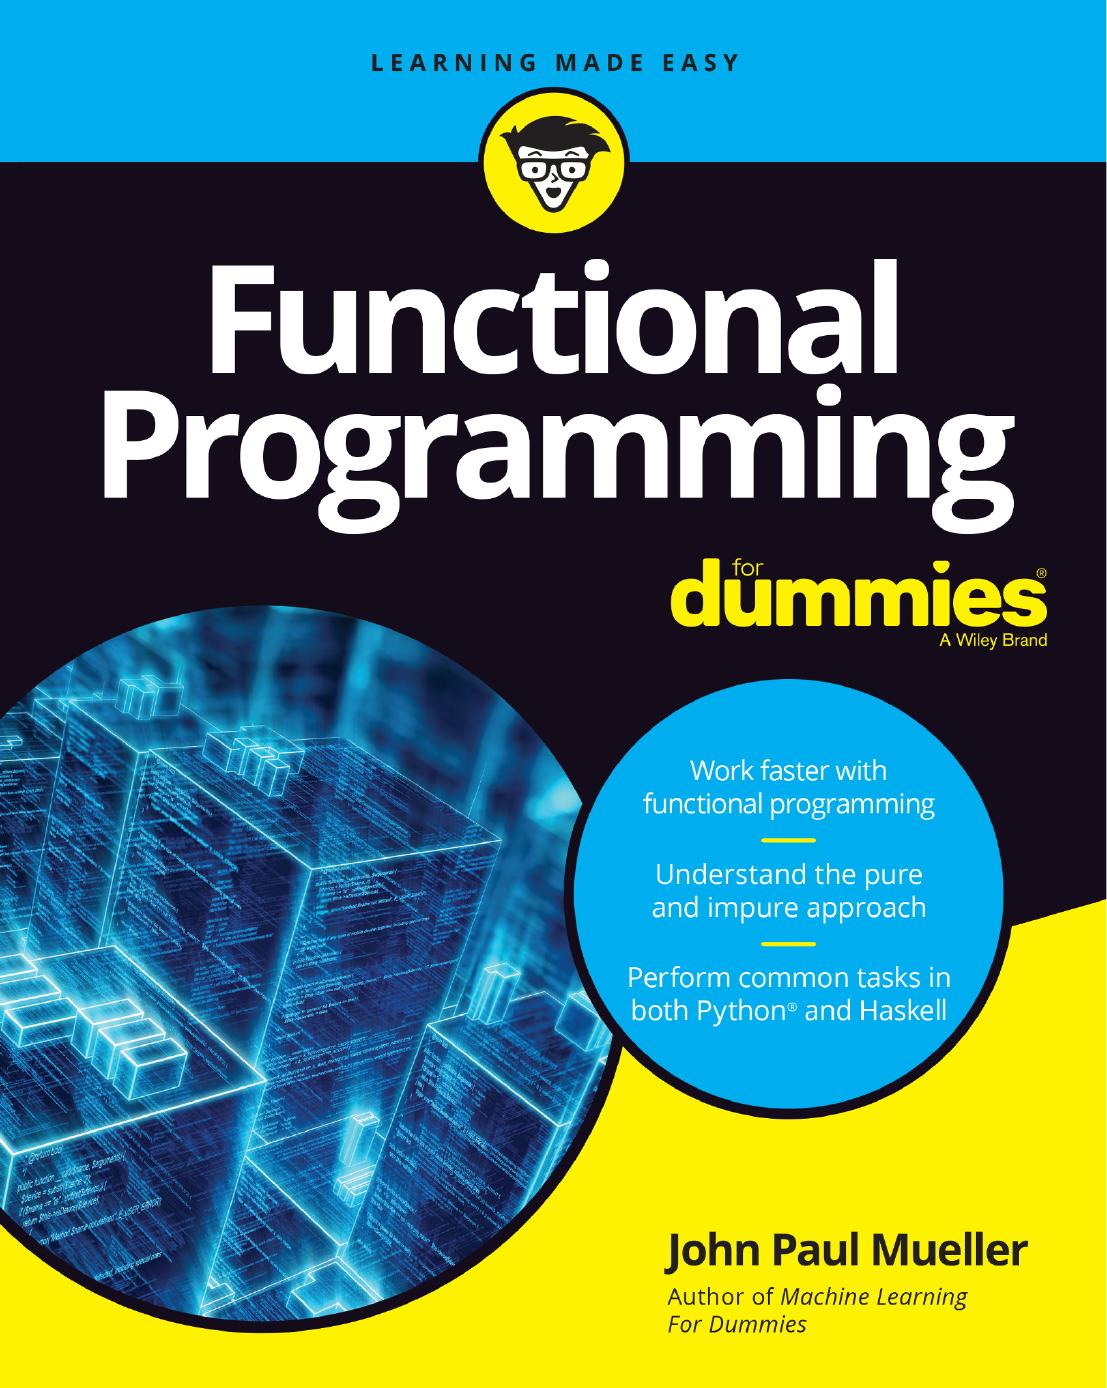
\includegraphics[height=0.2\textwidth]{./images/FunctionalProgrammingForDummies.jpeg}
		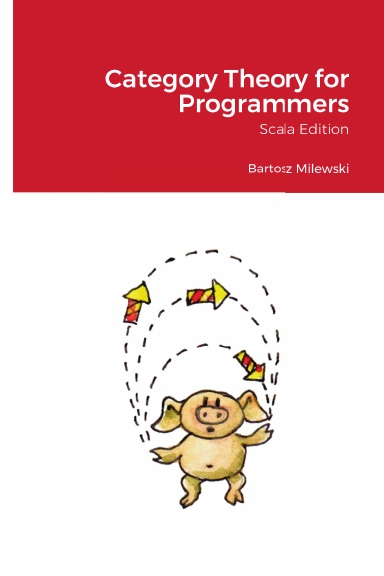
\includegraphics[height=0.2\textwidth]{./images/categoryTheoryForProgrammers.jpg}
	\end{center}
\end{frame}
